% ------------------------------------------------------------------------------
% TYPO3 Version 10.0 - What's New (English Version)
%
% @author	Michael Schams <schams.net>
% @license	Creative Commons BY-NC-SA 3.0
% @link		http://typo3.org/download/release-notes/whats-new/
% @language	English
% ------------------------------------------------------------------------------

\section{Änderungen für Entwickler}
\begin{frame}[fragile]
	\frametitle{Änderungen für Entwickler}

	\begin{center}\huge{Kapitel 4:}\end{center}
	\begin{center}\huge{\color{typo3darkgrey}\textbf{Änderungen für Entwickler}}\end{center}

\end{frame}

% ------------------------------------------------------------------------------
% TYPO3 Version 10.0 - Breaking Changes

\begin{frame}[fragile]
	\frametitle{Änderungen für Entwickler}
	\framesubtitle{Breaking Changes}

	\small
		Hinweis für Entwickler: in TYPO3 v9 wurden einige PHP-Klassen, Interfaces,
		Klassenaliase, Eigenschaften, Methoden, Konstanten, globale Optionen und Variablen 
		 usw. als veraltet markiert.

		\vspace{0.2cm}

		Entsprechend der \textbf{Deprecation} von TYPO3 wurden diese Komponenten
		in TYPO3 v10.0 entfernt.

		\vspace{0.2cm}

		Dies beinhaltet auch einige Hooks, PHP-Annotationen (wie zum Beispiel \texttt{@inject} und
		\texttt{@validate}), sowie einige geänderte Sichtbarkeiten (e.g. z.B. von
		"\texttt{public}" bis "\texttt{protected}").

		\vspace{0.2cm}

		Aktivieren Sie das Verfallsprotokoll und testen Sie Ihren Code sorgfältig 
		um mögliche Probleme zu ermitteln. Verwenden Sie den integrierten
		\href{https://docs.typo3.org/m/typo3/reference-coreapi/master/en-us/ApiOverview/ExtensionScanner/Index.html}{Extension Scanner} 
		um einen vollständigen Bericht über Erweiterungsinkompatibilitäten zu erhalten.

	\normalsize

\end{frame}

% ------------------------------------------------------------------------------
% Feature | 88643 | New Mail API based on symfony/mailer and symfony/mime
% Breaking | 88643 | Removed Swiftmailerswiftmailer Dependency

\begin{frame}[fragile]
	\frametitle{Änderungen für Entwickler}
	\framesubtitle{Neue Mail-API}

	\begin{itemize}
		\item SwiftMailer wurde durch modernere Bibliotheken ersetzt:

			\begin{itemize}
				\item \texttt{symfony/mime} zum Erstellen von E-Mail-Nachrichten
				\item \texttt{symfony/mailer} zum Versenden von E-Mails
			\end{itemize}

		\item Die PHP-Function \texttt{mail()} wird nicht mehr unterstützt.

			\begin{itemize}\smaller
				\item[\ding{228}] Es wird empfohlen zum \texttt{sendmail} oder \texttt{smtp} zu wechseln.
			\end{itemize}\normalsize

		\item Benutzerdefinierte SwiftMailer-Plugins oder -Transporte erfordern eine Migration.

		\item Sie finden weitere Infos zur Nutzung der neuen Mail-API-Funktionen in der \href{https://symfony.com/doc/current/mailer.html}{Symfony Dokumentation}.
	\end{itemize}

\end{frame}

% ------------------------------------------------------------------------------
% Feature | 84112 | Symfony dependency injection for core and Extbase

\begin{frame}[fragile]
	\frametitle{Änderungen für Entwickler}
	\framesubtitle{Symfony Dependency Management/Injection (1)}

	\begin{itemize}
		\item Das Paket \texttt{symfony/dependency-injection} wurde integriert und dient
			zur Verwaltung des systemweiten Abhängigkeitsmanagements und der Abhängigkeitsinjektion 
			für Klassen.

		\item Dieser Ansatz zielt darauf ab, den Extbase-Abhängigkeitsinjektionscontainer 
			und den Objektmanager zu ersetzen.

		\item Daher sollten Klassen angepasst und vermieden werden (wann immer möglich):

			\begin{itemize}\small
				\item \texttt{\textbackslash
					TYPO3\textbackslash
					CMS\textbackslash
					Extbase\textbackslash
					Object\textbackslash
					ObjectManager}
				\item \texttt{\textbackslash
					TYPO3\textbackslash
					CMS\textbackslash
					Core\textbackslash
					Utility\textbackslash
					GeneralUtility::makeInstance()}
			\end{itemize}\normalsize

	\end{itemize}

\end{frame}

% ------------------------------------------------------------------------------
% Feature | 84112 | Symfony dependency injection for core and Extbase

\begin{frame}[fragile]
	\frametitle{Änderungen für Entwickler}
	\framesubtitle{Symfony Dependency Management/Injection (2)}

	% decrease font size for code listing
	\lstset{basicstyle=\tiny\ttfamily}

	\begin{itemize}
		\item Mögliche Konfigurationsoptionen:

			\begin{itemize}
				\item Autowiring (s. Beispiel unten)
				\item Manual Wiring 
					(siehe \href{https://docs.typo3.org/c/typo3/cms-core/master/en-us/Changelog/10.0/Feature-84112-SymfonyDependencyInjectionForCoreAndExtbase.html}{Änderungsprotokoll})
				\item Erweiterte Funktionalität
					(siehe \href{https://docs.typo3.org/c/typo3/cms-core/master/en-us/Changelog/10.0/Feature-84112-SymfonyDependencyInjectionForCoreAndExtbase.html}{Änderungsprotokoll})
			\end{itemize}

		% \smaller For example "autowiring":\normalsize

\begin{lstlisting}
# Configuration/Services.yaml
services:
  _defaults:
    autowire: true
    autoconfigure: true
    public: false

  Your\Namespace\:
    resource: '../Classes/*'
\end{lstlisting}

		\item Siehe die \href{https://symfony.com/doc/current/service_container.html}{Symfony Dokumentation} für weitere Details.

	\end{itemize}

\end{frame}

% ------------------------------------------------------------------------------
% Feature | 88769 | Introduce a generic EventDispatcher based on PSR-14
% Feature | 88770 | Add PSR-14 EventDispatcher logic based on DI

\begin{frame}[fragile]
	\frametitle{Änderungen für Entwickler}
	\framesubtitle{Event Dispatching (1)}

	\begin{itemize}
		\item Ein neues "EventDispatcher" -System wurde hinzugefügt, um die aktuellen
			Hooks und Signal/Slots-Konzepte zu ersetzen.

		\item Es basiert auf dem \href{https://www.php-fig.org/psr/psr-14}{PSR-14 Standard}:
			mit dem Entwickler auf einfache und konsistente Weise Logik in eine Anwendung einfügen können.

		\item PSR-14 besteht aus den folgenden vier Komponenten:

			\begin{itemize}
				\item Ein \textbf{EventDispatcher}-Objekt, mit dem ein Ereignis ausgelöst wird.
				\item Ein \textbf{ListenerProvider}-Objekt: enthält registrierte Listener für alle Ereignisse.
				\item Ein oder mehrere \textbf{Event}-Objekte, die vom TYPO3 Core oder Extensions ("Emitter") aufgerufen werden.
				\item Ein oder mehrere \textbf{Listener}, die registriert sind (in der Regel in Erweiterungen und PHP-Paketen).
			\end{itemize}

% Short-Term goal is to deprecate SignalSlot dispatcher in TYPO3 v10,
% and migrate all signals to the EventDispatcher.

	\end{itemize}

\end{frame}

% ------------------------------------------------------------------------------
% Feature | 88769 | Introduce a generic EventDispatcher based on PSR-14
% Feature | 88770 | Add PSR-14 EventDispatcher logic based on DI

\begin{frame}[fragile]
	\frametitle{Änderungen für Entwickler}
	\framesubtitle{Event Dispatching (2)}

	% decrease font size for code listing
	\lstset{basicstyle=\tiny\ttfamily}

	Implementierungsbeispiel:

	\begin{itemize}\smaller
		\item[\ding{202}] Fügen Sie der Datei \texttt{Configuration/Services.yaml} den Tag \texttt{event.listener} hinzu:

\begin{lstlisting}
services:
  Vendor\Example\EventListener\NullMailer:
    tags:
      - { name: event.listener, identifier: 'myListener', event: TYPO3\CMS\Core\Mail\Event\AfterMailerInitializationEvent, before: 'redirects, anotherIdentifier' }
\end{lstlisting}

		\item[\ding{203}] Implementieren Sie Ihr Ereignisobjekt:

\begin{lstlisting}
namespace Vendor\Example\EventListener;

class NullMailer
{
  public function __invoke(AfterMailerInitializationEvent $event): void
  {
    $event->getMailer()->injectMailSettings(['transport' => 'null']);
  }
}
\end{lstlisting}

	\end{itemize}\normalsize

\end{frame}

% ------------------------------------------------------------------------------
% Feature | 88769 | Introduce a generic EventDispatcher based on PSR-14
% Feature | 88770 | Add PSR-14 EventDispatcher logic based on DI

\begin{frame}[fragile]
	\frametitle{Änderungen für Entwickler}
	\framesubtitle{Event Dispatching (3)}

	% decrease font size for code listing
	\lstset{basicstyle=\tiny\ttfamily}

	\begin{itemize}
		\item Im Backend kann man auf die Liste der verfügbaren Event Listener zugreifen:\newline
			\smaller
				(erfordert die Systemerweiterung \texttt{EXT:lowlevel})
			\normalsize
	\end{itemize}

	\begin{figure}
		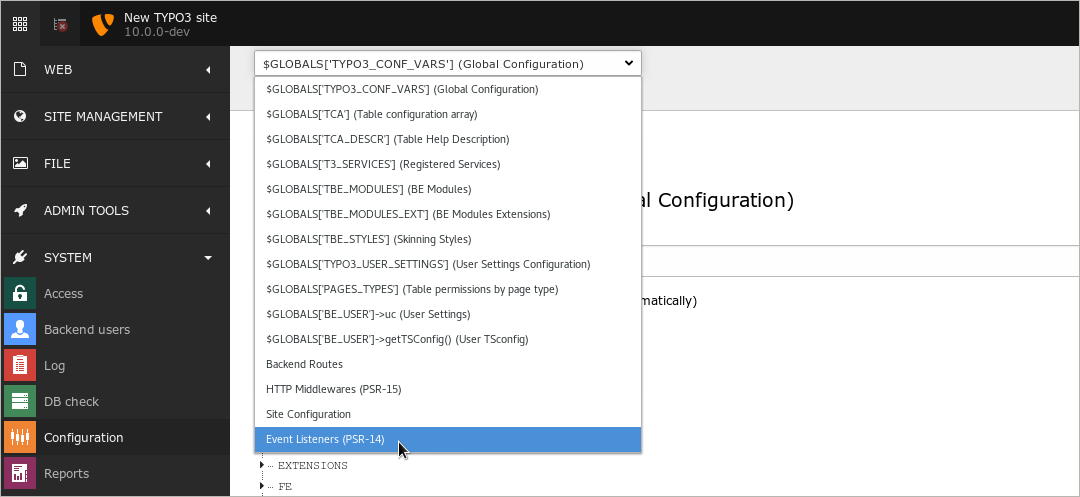
\includegraphics[width=0.70\linewidth]{ChangesForDevelopers/88770-PSR14-EventDispatcher.png}
	\end{figure}

\end{frame}


% ------------------------------------------------------------------------------
% Feature | 88769 | Introduce a generic EventDispatcher based on PSR-14
% Feature | 88770 | Add PSR-14 EventDispatcher logic based on DI

\begin{frame}[fragile]
	\frametitle{Änderungen für Entwickler}
	\framesubtitle{Event Dispatching (4)}

	% decrease font size for code listing
	\lstset{basicstyle=\tiny\ttfamily}

	\begin{itemize}
		\item Best Practices:

			\begin{itemize}
				\item Fügen Sie nur einen Listener pro PHP-Klasse hinzu und verwenden Sie \texttt{\_\_invoke()} als Methodenname.
				\item Fügen Sie dem Klassennamen das Suffix "\texttt{Event}" hinzu, wenn Sie eine neue Event-PHP-Klasse erstellen.
				\item Verschieben Sie die Event PHP-Klassendatei in einen geeigneten Ordner, zum Beispiel \texttt{Classes/Database/Event}.
				\item Verwenden Sie die Abhängigkeitsinjektion in Form eines Kontruktorarguments, um das 
					EventDispatcher-Objekt zu empfangen, sofern dies möglich ist.
			\end{itemize}

		\item Zusätzliche Anmerkung:\newline
			\small
				Ereignisse, die vom TYPO3-Core bereitgestellt werden, richten sich nach der Verfallsrichtlinie von TYPO3, mit Ausnahme der Konstruktorargumente,
				die davon abweichen können.
			\normalsize

	\end{itemize}

\end{frame}

% ------------------------------------------------------------------------------
% Feature | 88799 | Use PSR-3 interface for logging

\begin{frame}[fragile]
	\frametitle{Änderungen für Entwickler}
	\framesubtitle{PSR-3 Logging Schnittstelle}

	\begin{itemize}
		\item Das Logging Framework von TYPO3 (insbesondere LogLevel und LogManage) verwendet jetzt die 
			\href{https://www.php-fig.org/psr/psr-3/}{PSR-3 Logger Schnittstelle}.

		\item PSR-3 ist eine standardisierte Methode,  mit der Bibliotheken ein
			\texttt{Psr\textbackslash
				Log\textbackslash
				LoggerInterface}-Objekt empfangen und einfach und global Protokolle darauf schreiben können.

			\item Auf diese Weise können Entwickler benutzerdefinierte Protokollfunktionen 
				verwenden und mit anderen Protokollierungssystemen interagieren.

	\end{itemize}

\end{frame}

% ------------------------------------------------------------------------------
% Breaking | 88182 | jsfunc.inline.js has been dropped
% Breaking | 88427 | jsfunc.evalfield.js has been removed
% Breaking | 88667 | Removed additionalJavaScriptSubmit from FormEngine
% Deprecation | 88433 | Deprecate top.openUrlInWindow

\begin{frame}[fragile]
	\frametitle{Veraltete/entfernte Funktionen}
	\framesubtitle{JavaScript Optionen und Funktionen (1)}

	\begin{itemize}
		\item Die folgenden JavaScript-Dateien wurden entfernt:

			\begin{itemize}
				\item \texttt{jsfunc.inline.js}
				\item \texttt{jsfunc.evalfield.js}
			\end{itemize}

			\begin{itemize}\smaller
				\item[\ding{228}] Verwenden Sie stattdessen \texttt{TYPO3/CMS/Backend/FormEngineValidation} 
			\end{itemize}\normalsize

		\item Zusätzliche Submit-Handler konnten zuvor durch die Option  \texttt{additionalJavaScriptSubmit}.
			hinzugefügt werden. Diese Option wurde entfernt.

			\begin{itemize}\smaller
				\item[\ding{228}] Erstellen Sie stattdessen ein AMD-Modul.
			\end{itemize}\normalsize

		\item Die globale JavaScript-Funktion \texttt{top.openUrlInWindow()} wurde als veraltet markiert.

	\end{itemize}

\end{frame}

% ------------------------------------------------------------------------------
% Breaking | 88411 | TBE_EDITOR.typo3form removed
% Deprecation | 88432 | Replaced md5js with an AMD module
% Deprecation | 88428 | top.rawurlencode and top.str_replace
% Deprecation | 88651 | Replace TYPO3/CMS/Backend/SplitButtons with TYPO3/CMS/Backend/DocumentSaveActions

\begin{frame}[fragile]
	\frametitle{Veraltete/Entfernte Funktionen}
	\framesubtitle{JavaScript Optionen und Funktionen (2)}

	\begin{itemize}

		\item Das globale Objekt \texttt{TBE\_EDITOR.typo3form} und seine Methoden \texttt{typo3FormFieldSet} und 
			\texttt{typo3FormFieldGet} wurden entfernt.

		\item Die Datei \texttt{md5.js} wurde als veraltet markiert.

			\begin{itemize}\smaller
				\item[\ding{228}] Laden Sie stattdessen das AMD-Modul \texttt{TYPO3/CMS/Backend/Hashing/Md5} via RequireJS.
			\end{itemize}\normalsize

		\item Die folgenden globalen JavaScript-Funktionen wurden als veraltet markiert:

		\begin{itemize}
			\item \texttt{top.rawurlencode()}
			\item \texttt{top.str\_replace()}
		\end{itemize}

		\item Das Modul \texttt{TYPO3/CMS/Backend.SplitButtons} wurde als veraltet markiert.

			\begin{itemize}\smaller
				\item[\ding{228}] Verwenden Sie stattdessen \texttt{TYPO3/CMS/Backend/DocumentSaveActions}.
			\end{itemize}\normalsize

 	\end{itemize}

\end{frame}

% ------------------------------------------------------------------------------
% Important | 87894 | Removed PHP Dependency algo26-matthiasidna-convert

\begin{frame}[fragile]
	\frametitle{Änderungen für Entwickler}
	\framesubtitle{UTF-8-basierte Domains}

	\begin{itemize}
		\item PHP bietet die Möglichkeit, Domains von UTF-8 in IDNA ASCII Form (“punicode”) zu konvertieren,
			zum Beispiel \href{https://www.php.net/manual/en/function.idn-to-ascii.php}{idn\_to\_ascii()}.

		\item Diese können direkt verwendet werden, wenn die PHP-Erweiterung
			"\href{https://www.php.net/manual/en/book.intl.php}{intl}" installiert wird.

		\item Wenn die PHP-Erweiterung nicht installiert ist, bietet das Paket \texttt{symfony/polyfill-intl-idn}
			diese Möglichkeit.

		\item Bisher wurde das jetzt entfernte Paket \texttt{algo26-matthias/idna-convert} verwendet.

	\end{itemize}

\end{frame}

% ------------------------------------------------------------------------------
% Feature | 87665 | Introduce BitSet class

\begin{frame}[fragile]
	\frametitle{Änderungen für Entwickler}
	\framesubtitle{BitSet Klasse}

	% decrease font size for code listing
	\lstset{basicstyle=\tiny\ttfamily}

	\begin{itemize}
		\item Um boolesche Flags effizient zu behandeln, wurde eine neue Klasse eingeführt:\newline
			\texttt{TYPO3\textbackslash
				CMS\textbackslash
				Core\textbackslash
				Type\textbackslash
				BitSet}

		\item Zum Beispiel:

\begin{lstlisting}
define('PERMISSIONS_NONE', 0b0); // 0
define('PERMISSIONS_PAGE_SHOW', 0b1); // 1
define('PERMISSIONS_PAGE_EDIT', 0b10); // 2
define('PERMISSIONS_PAGE_DELETE', 0b100); // 4
define('PERMISSIONS_PAGE_NEW', 0b1000); // 8
define('PERMISSIONS_CONTENT_EDIT', 0b10000); // 16
define('PERMISSIONS_ALL', 0b11111); // 31

$bitSet = new \TYPO3\CMS\Core\Type\BitSet(PERMISSIONS_PAGE_SHOW | PERMISSIONS_PAGE_NEW);
$bitSet->get(PERMISSIONS_PAGE_SHOW); // true
$bitSet->get(PERMISSIONS_CONTENT_EDIT); // false
\end{lstlisting}

	\end{itemize}

\end{frame}

% ------------------------------------------------------------------------------
% Important | 87516 | Remove Core HTTP Request Handler Interface

\begin{frame}[fragile]
	\frametitle{Änderungen für Entwickler}
	\framesubtitle{Request Handler (1)}

	\begin{itemize}
		\item Die folgende interne Schnittstelle wurde zugunsten von
			PSR-15-Request-Handler- und Middleware-Schnittstellen entfernt:\newline
			\texttt{TYPO3\textbackslash
				CMS\textbackslash
				Core\textbackslash
				Http\textbackslash
				RequestHandlerInterface}

	\end{itemize}

\end{frame}

% ------------------------------------------------------------------------------
% Breaking | 88687 | Configure extbase request handlers via PHP

\begin{frame}[fragile]
	\frametitle{Änderungen für Entwickler}
	\framesubtitle{Request Handler (2)}

	% decrease font size for code listing
	\lstset{basicstyle=\tiny\ttfamily}

	\begin{itemize}
		\item Die Konfiguration von Extbase-Request-Handlern ist mit TypoScript nicht mehr möglich.

		\smaller\ Die alte Methode in TypoScript:\normalsize
\begin{lstlisting}
config.tx_extbase {
  mvc {
    requestHandlers {
      Vendor\Example\Mvc\Web\FrontendRequestHandler = Vendor\Example\Mvc\Web\FrontendRequestHandler
    }
  }
}
\end{lstlisting}

		\smaller\ Die neue Methode in der Datei \texttt{Configuration/Extbase/RequestHandlers.php}:\normalsize
\begin{lstlisting}
<?php
declare(strict_types = 1);

return [
  \Vendor\Example\Mvc\Web\FrontendRequestHandler::class,
];
\end{lstlisting}

	\end{itemize}

\end{frame}


% ------------------------------------------------------------------------------
% Deprecation | 88366 | Default caching framework cache names changed

\begin{frame}[fragile]
	\frametitle{Änderungen für Entwickler}
	\framesubtitle{Caching-Framework}

	% decrease font size for code listing
	\lstset{basicstyle=\tiny\ttfamily}

	\begin{itemize}
		\item Folgende Caches wurden umbenannt:

			\begin{itemize}\smaller
				\item \texttt{cache\_core} \textrightarrow\hspace{0.1cm}\texttt{core}
				\item \texttt{cache\_hash} \textrightarrow\hspace{0.1cm}\texttt{hash}
				\item \texttt{cache\_pages} \textrightarrow\hspace{0.1cm}\texttt{pages}
				\item \texttt{cache\_pagesection} \textrightarrow\hspace{0.1cm}\texttt{pagesection}
				\item \texttt{cache\_runtime} \textrightarrow\hspace{0.1cm}\texttt{runtime}
				\item \texttt{cache\_rootline} \textrightarrow\hspace{0.1cm}\texttt{rootline}
				\item \texttt{cache\_imagesizes} \textrightarrow\hspace{0.1cm}\texttt{imagesizes}
			\end{itemize}\normalsize

		\item Neue Methode um auf Caches zuzugreifen:

\begin{lstlisting}
OLD:
$cacheManager->getCache('cache_core').

NEW:
$cacheManager->getCache('core')
\end{lstlisting}

		\item Das Präfix \texttt{cf\_}  wurde aus den Datenbanktabellen entfernt.
	\end{itemize}

\end{frame}

% ------------------------------------------------------------------------------
% Deprecation | 87550 | Use controller classes when registering plugins/modules

\begin{frame}[fragile]
	\frametitle{Änderungen für Entwickler}
	\framesubtitle{Extbase und Fluid}

	% decrease font size for code listing
	\lstset{basicstyle=\tiny\ttfamily}

	\begin{itemize}
		\item Das Registrieren von Plugins/Modulen erfordert nun vollständig qualifizierte Klassennamen

			\begin{itemize}\smaller
				\item \texttt{\textbackslash
					TYPO3\textbackslash
					CMS\textbackslash
					Extbase\textbackslash
					Utility\textbackslash
					ExtensionUtility::configurePlugin()}
				\item \texttt{\textbackslash
					TYPO3\textbackslash
					CMS\textbackslash
					Extbase\textbackslash
					Utility\textbackslash
					ExtensionUtility::registerModule()}
			\end{itemize}\normalsize

		\item Lassen Sie auch den Herstellernamen im Erweiterungsnamen weg (erstes Argument).

			\begin{itemize}\smaller
				\item[\ding{228}] Verwenden Sie "\texttt{ExampleBlog}" anstelle von "\texttt{Vendor.ExampleBlog}".
			\end{itemize}

		\item Zum Beispiel:

\begin{lstlisting}
\TYPO3\CMS\Extbase\Utility\ExtensionUtility::configurePlugin(
  'ExampleBlog', // previously: 'Vendor.ExampleBlog'
  'pi1',
  [
    \Vendor\Example\Controller\BlogController::class => 'list,update,delete'
  ],
  [
    \Vendor\Example\Controller\BlogController::class => 'list,update,delete'
  ]
);
\end{lstlisting}

	\end{itemize}

\end{frame}

% ------------------------------------------------------------------------------
% Breaking | 87627 | Remove Property extensionName of AbstractController

\begin{frame}[fragile]
	\frametitle{Veraltete/Entfernte Funktionen}
	\framesubtitle{Extbase und Fluid}

	\begin{itemize}
		\item Die Eigentschaft \texttt{extensionName} von AbstractController wurde entfernt.

			\begin{itemize}\smaller
				\item[\ding{228}] Verwenden Sie stattdessen \texttt{\textbackslash
					TYPO3\textbackslash
					CMS\textbackslash
					Extbase\textbackslash
					Mvc\textbackslash
					Request::getControllerExtensionName()}.
			\end{itemize}\normalsize

	\end{itemize}

\end{frame}

% ------------------------------------------------------------------------------
% Feature | 87457 | Use symfony/propertyinfo to gather doc block information

\begin{frame}[fragile]
	\frametitle{Änderungen für Entwickler}
	\framesubtitle{Extbase and Fluid}

	% decrease font size for code listing
	\lstset{basicstyle=\tiny\ttfamily}

	\begin{itemize}
		\item Extbase-Modelle unterstützen jetzt nicht vollständig qualifizierte Klassennamen in DocBlocks.

\begin{lstlisting}
use TYPO3\CMS\Extbase\Persistence\ObjectStorage;
use ExtbaseTeam\BlogExample\Domain\Model\Comment;

class Post
{
  /**
   * @var ObjectStorage<Comment>
   */
  public $comments;
}
\end{lstlisting}

	\end{itemize}

\end{frame}

% ------------------------------------------------------------------------------
% Breaking | 87957 | Validators are not registered automatically in Extbase anymore

\begin{frame}[fragile]
	\frametitle{Änderungen für Entwickler}
	\framesubtitle{Extbase and Fluid}

	% decrease font size for code listing
	\lstset{basicstyle=\tiny\ttfamily}

	\begin{itemize}
		\item Validatoren werden nicht mehr automatisch in Extbase registriert.
		\item Für ein Model mit dem Namen
			\small\texttt{Vendor\textbackslash
				Example\textbackslash
				Domain\textbackslash
				Model\textbackslash
				Blog}\normalsize,\newline
			verwendet Extbase automatisch den Validator
			\small\texttt{Vendor\textbackslash
				Example\textbackslash
				Domain\textbackslash
				Validator\textbackslash
				BlogValidator}\normalsize

		\item Validatoren müssen jetzt manuell registriert werden:

\begin{lstlisting}
use Vendor\Example\Domain\Model\Blog;
use TYPO3\CMS\Extbase\Annotation as Extbase;
use TYPO3\CMS\Extbase\Mvc\Controller\ActionController;

class BlogController extends ActionController
{
  /**
   * @Extbase\Validate(param="blog", validator="Vendor\Example\Domain\Validator\BlogValidator")
   */
  public function showAction(Blog $blog)
  {
    // ...
  }
}
\end{lstlisting}

	\end{itemize}

\end{frame}

% ------------------------------------------------------------------------------
% Breaking | 87623 | Replace config.persistence.classes typoscript configuration (1)

\begin{frame}[fragile]
	\frametitle{Änderungen für Entwickler}
	\framesubtitle{Extbase and Fluid - Klassenzuordnung (1)}

	% decrease font size for code listing
	\lstset{basicstyle=\tiny\ttfamily}

	\begin{itemize}
		\item Persistenzbezogene Klassenzuordnung mit TypoScript wird nicht mehr unterstützt:

\begin{lstlisting}
config.tx_example_blog {
  persistence {
    classes {
      Vendor\Example\Domain\Model\Author {
        mapping {
          tableName = fe_users
          columns.name.mapOnProperty = fullname
        }
      }
    }
  }
}
\end{lstlisting}

	\end{itemize}

\end{frame}

% ------------------------------------------------------------------------------
% Breaking | 87623 | Replace config.persistence.classes typoscript configuration (2)

\begin{frame}[fragile]
	\frametitle{Änderungen für Entwickler}
	\framesubtitle{Extbase and Fluid - Klassenzuordnung (2)}

	% decrease font size for code listing
	\lstset{basicstyle=\tiny\ttfamily}

	\begin{itemize}
		\item Das Mapping muss in einer PHP-Datei implementiert werden \texttt{Configuration/Extbase/Persistence/Classes.php}:

\begin{lstlisting}
<?php
declare(strict_types = 1);

return [
  \Vendor\Example\Domain\Model\Author::class => [
    'tableName' => 'fe_users',
    'properties' => [
      'fullname' => [
        'fieldName' => 'name'
      ]
    ]
  ]
];
\end{lstlisting}

		\begin{itemize}\smaller
			\item[\ding{228}] beachten Sie, dass der Eigenschaftsname und das DB-Feld vertauscht wurden!\newline
				Vorher:\tabto{1.6cm}\texttt{<db-field>.mapOnProperty = <property>}\newline
				Jetzt:\tabto{1.6cm}\texttt{properties.<property>.fieldname = <db-field>}
		\end{itemize}\normalsize

	\end{itemize}

\end{frame}

% ------------------------------------------------------------------------------
% Breaking | 87594 | Harden Extbase

\begin{frame}[fragile]
	\frametitle{Änderungen für Entwickler}
	\framesubtitle{Extbase and Fluid}

	% decrease font size for code listing
	\lstset{basicstyle=\smaller\ttfamily}

	\begin{itemize}
		\item Es gibt nun in Klassendateien den Modus "strict type" und Type Hints für Skalare.

\begin{lstlisting}
<?php
declare(strict_types=1);
\end{lstlisting}

		% Method signatures in Extbase classes have been updated.
		\item Dies führt zu schwerwiegenden PHP-Fehlern, wenn die Methodensignaturen in benutzerdefinierten
			  Erweiterungen nicht mit den Schnittstellen und/oder übergeordneten Klassen kompatibel sind.

		\item Siehe \href{https://forge.typo3.org/issues/87594}{forge \#87594}
			für eine vollständige Liste der Änderungen.

		\item Diese Aufgabe ist aktuell noch in Bearbeitung und es werden weitere Änderungen vorgenommen werden.

	\end{itemize}

\end{frame}

% ------------------------------------------------------------------------------
% Breaking | 87937 | TCA option selicon_field_path removed
% Breaking | 87989 | TCA option setToDefaultOnCopy removed
% Breaking | 87936 | TCA for sys_history removed

\begin{frame}[fragile]
	\frametitle{Änderungen für Entwickler}
	\framesubtitle{TCA Änderungen}

	\begin{itemize}
		\item Die folgenden TCA-Optionen wurden entfernt:

			\begin{itemize}
				\item \texttt{\$TCA[\$tableName]['ctrl']['selicon\_field\_path']}
				\item \texttt{\$TCA[\$tableName]['ctrl']['setToDefaultOnCopy']}
			\end{itemize}

			\begin{itemize}\smaller
				\item[\ding{228}] Beim Kopieren von Datensätzen sollte ein DataHandler verwendet werden um die Felder zurückzusetzen.
			\end{itemize}\normalsize

		\item Das gesamte TCA von \texttt{sys\_history} wurde entfernt und das Datenbankfeld \texttt{pid} wurde gelöscht.
			Der Zugriff auf \texttt{\$GLOBALS['TCA']['sys\_history']} löst eine PHP-Warnung aus.

	\end{itemize}

\end{frame}

% ------------------------------------------------------------------------------
% Breaking | 88527 | Overriding custom values in User Authentication derivatives

\begin{frame}[fragile]
	\frametitle{Änderungen für Entwickler}
	\framesubtitle{Benutzerauthentifizierungsklassen / -dienste (1)}

	\begin{itemize}
		\item Die folgende abstrakte Klasse wurde umstrukturiert:\newline
			\small\texttt{TYPO3\textbackslash
				CMS\textbackslash
				Core\textbackslash
				Authentication\textbackslash
				AbstractUserAuthentication}\normalsize
		\item Dies umfasst auch die folgenden zwei direkten Unterklassen:

			\begin{itemize}
				\item \texttt{BackendUserAuthentication}
				\item \texttt{FrontendUserAuthentication}
			\end{itemize}

		\item Diese Änderung wirkt sich auf folgende Eigenschaften aus:

			\begin{itemize}
				\item \texttt{sessionTimeout}
				\item \texttt{gc\_time}
				\item \texttt{sessionDataLifetime}
				\item \texttt{loginType}
			\end{itemize}

	\end{itemize}

\end{frame}

% ------------------------------------------------------------------------------
% Breaking | 88646 | Removed inheritance of AbstractService from AbstractAuthenticationService

\begin{frame}[fragile]
	\frametitle{Änderungen für Entwickler}
	\framesubtitle{Benutzerauthentifizierungsklassen / -dienste (2)}

	\begin{itemize}

		\item Die folgende Klasse erbt nicht mehr von 
			\smaller\texttt{AbstractService}\normalsize\hspace{0.1cm}:
			\smaller\texttt{\textbackslash
				TYPO3\textbackslash
				CMS\textbackslash
				Core\textbackslash
				Authentication\textbackslash
				AbstractAuthenticationService}\normalsize

		\item Dies beeinträchtigt möglicherweise einige der verfügbaren Hooks und benutzerdefinierten Authentifizierungsanbieter.

		\item Entwickler werden gebeten, ihre individuellen Authentifizierungsdienste zu überprüfen 
			und ihren Code zu aktualisieren, falls erforderlich.

	\end{itemize}

\end{frame}

% ------------------------------------------------------------------------------
% Deprecation | 87882 | File related controllers moved to EXT:filelist

\begin{frame}[fragile]
	\frametitle{Änderungen für Entwickler}
	\framesubtitle{Dateilisten-Controller}

	\begin{itemize}
		\item Die folgenden Controller wurden nach  \texttt{EXT:filelist} verschoben:

			\begin{itemize}\small
				\item \texttt{CreateFolderController}
				\item \texttt{EditFileController}
				\item \texttt{FileUploadController}
				\item \texttt{RenameFileController}
				\item \texttt{ReplaceFileController}
			\end{itemize}\normalsize

		\item Infolgedessen wurde der Namespace auch geändert\newline
			\texttt{\textbackslash
				TYPO3\textbackslash
				CMS\textbackslash
				Filelist\textbackslash
				Controller\textbackslash
				File}

		\vspace{0.2cm}

		\small
			Hinweis: Verwenden Sie TYPO3 FAL als API und fügen Sie Ihre 
			eigenen Funktionen mit Ihrem eigenen Controller hinzu, anstatt die oben genannten
			\textbf{internen} Controller wiederzuverwenden.
		\normalsize

	\end{itemize}

\end{frame}

% ------------------------------------------------------------------------------
% Deprecation | 88499 | BackendUtility::getViewDomain()

\begin{frame}[fragile]
	\frametitle{Änderungen für Entwickler}
	\framesubtitle{Frontend Vorschau URL}

	% decrease font size for code listing
	\lstset{basicstyle=\tiny\ttfamily}

	\begin{itemize}
		\item Die folgende statische Methode wurde als veraltet markiert:\newline
			\smaller\texttt{\textbackslash
				TYPO3\textbackslash
				CMS\textbackslash
				Backend\textbackslash
				Utility\textbackslash
				BackendUtility::getViewDomain()}\normalsize

		\item Ersetzen Sie die Methode, indem Sie eine Seite anhand einer bestimmten Seiten-ID im TYPO3-Backend direkt erkennen.
		\item Zum Beispiel:

\begin{lstlisting}
$pageId = 123;
$site = GeneralUtility::makeInstance(SiteFinder::class)->getSiteByPageId($pageId);
$url = $site->getRouter()->generateUri($pageId, ['type' => 13]);
\end{lstlisting}

	\end{itemize}

\end{frame}

% ------------------------------------------------------------------------------
% Deprecation | 88406 | setCacheHash/noCacheHash options in ViewHelpers and UriBuilder

\begin{frame}[fragile]
	\frametitle{Änderungen für Entwickler}
	\framesubtitle{cHash in UriBuilder und ViewHelpers}

	% decrease font size for code listing
	\lstset{basicstyle=\smaller\ttfamily}

	\begin{itemize}
		\item Die folgenden beiden Extbase UriBuilder-Methoden sind veraltet:

			\begin{itemize}
				\item \texttt{UriBuilder->setUseCacheHash()}
				\item \texttt{UriBuilder->getUseCacheHash()}
			\end{itemize}

		\item Dies wirkt sich auch auf eine Reihe von Fluid ViewHelpers aus:
	\end{itemize}
	\vspace{-0.4cm}
	\begin{columns}[T]
		\begin{column}{.05\textwidth}
		\end{column}
		\begin{column}{.45\textwidth}
			\begin{itemize}\smaller
				\item \texttt{f:form}
				\item \texttt{f:link.action}
				\item \texttt{f:link.page}
				\item \texttt{f:link.typolink}
				\item \texttt{f:uri.action}
			\end{itemize}\normalsize
		\end{column}
		\begin{column}{.45\textwidth}
			\begin{itemize}\smaller
				\item \texttt{f:uri.page}
				\item \texttt{f:uri.typolink}
				\item \texttt{f:widget.link}
				\item \texttt{f:widget.uri}
			\end{itemize}\normalsize
		\end{column}
	\end{columns}
	\vspace{0.2cm}
	\begin{itemize}
		\item ..... sowie auf die TypoLink Option "\texttt{useCacheHash}".
	\end{itemize}

\end{frame}

% ------------------------------------------------------------------------------
% Breaking | 88540 | Changed Request Workflow for Frontend Requests

\begin{frame}[fragile]
	\frametitle{Änderungen für Entwickler}
	\framesubtitle{Frontend Request Workflow}

	% decrease font size for code listing
	\lstset{basicstyle=\smaller\ttfamily}

	\begin{itemize}
		\item Der Frontend Request Workflow wurde erheblich überarbeitet.

		\item Seit TYPO3 v9 werden alle beteiligten Komponenten mit PSR-15-Middleware, PSR-15-Request-Handler und 
			TypoScriptFrontendController (TSFE) erstellt.

		\item Dies wirkt sich auf benutzerdefinierten Code aus, wenn der folgende Hook und eine Frontend-Sitzung verwendet werden:\newline
			{\fontsize{7}{8}\selectfont\texttt{\$GLOBALS['TYPO3\_CONF\_VARS']['SC\_OPTIONS']['tslib/class.tslib\_fe.php']['hook\_eofe']}}

			\begin{itemize}\smaller
				\item[\ding{228}] Verwenden Sie eine PSR-15-Middleware anstelle eines Hooks, oder rufen Sie in PHP \texttt{storeSessionData}
				innerhalb des Hooks auf.
			\end{itemize}\normalsize

	\end{itemize}

\end{frame}

% ------------------------------------------------------------------------------
% Breaking | 88498 | Global data for TimeTracker statistics removed

\begin{frame}[fragile]
	\frametitle{Änderungen für Entwickler}
	\framesubtitle{Frontend Request Workflow}

	% decrease font size for code listing
	\lstset{basicstyle=\smaller\ttfamily}

	\begin{itemize}
		\item Die folgenden globalen Variablen wurden entfernt:

			\begin{itemize}
				\item \texttt{\$GLOBALS['TYPO3\_MISC']['microtime\_start']}
				\item \texttt{\$GLOBALS['TYPO3\_MISC']['microtime\_end']}
				\item \texttt{\$GLOBALS['TYPO3\_MISC']['microtime\_BE\_USER\_start']}
				\item \texttt{\$GLOBALS['TYPO3\_MISC']['microtime\_BE\_USER\_end']}
			\end{itemize}

		\item Der TYPO3-Core verwendete sie beispielsweise im Admin-Panel und im HTTP-Header.

			\begin{itemize}\smaller
				\item[\ding{228}] Verwenden Sie stattdessen \texttt{TimeTracker->finish()}.
			\end{itemize}\normalsize

	\end{itemize}

\end{frame}


% ------------------------------------------------------------------------------
% Deprecation | 88569 | Locales::initialize() in favor of regular singleton instance
% Deprecation | 88473 | TypoScriptFrontendController->settingLocale

\begin{frame}[fragile]
	\frametitle{Veraltete/Entfernte Funktionen}
	\framesubtitle{Locales}

	\begin{itemize}
		\item Die Methode \texttt{Locales::initialize()} wurde als veraltet markiert.

			\begin{itemize}\smaller
				\item[\ding{228}] Verwenden Sie stattdessen \texttt{GeneralUtility::makeInstance(Locales::class)} oder
				Dependency Injection, um eine Instanz der Klasse \texttt{Locales} abzurufen.
			\end{itemize}\normalsize

		\item Die Funktionalität folgender Methode wurde als veraltet markiert:\newline
			\texttt{TypoScriptFrontendController->settingLocale()}.

			\begin{itemize}\smaller
				\item[\ding{228}] Die Funktion ist nun verfügbar als
				{\fontsize{8}{8} \selectfont \texttt{Locales::setSystemLocaleFromSiteLanguage()}.}
			\end{itemize}\normalsize

	\end{itemize}

\end{frame}

% ------------------------------------------------------------------------------
% Deprecation | 88559 | TSFE->sys_language_isocode

\begin{frame}[fragile]
	\frametitle{Veraltete/Entfernte Funktionen}
	\framesubtitle{Locales}

	\begin{itemize}
		\item Public property \texttt{TypoScriptFrontendController->sys\_language\_isocode}
			wurde als veraltet markiert.

			\begin{itemize}\smaller
				\item[\ding{228}] Greifen Sie stattdessen über \texttt{SiteLanguage->getTwoLetterIsoCode()}
				und \texttt{sitelanguage:twoLetterIsoCode} auf die Eigenschaft zu.
			\end{itemize}\normalsize

	\end{itemize}

\end{frame}

% ------------------------------------------------------------------------------
% Breaking | 88458 | Removed Frontend Track User ftu functionality

\begin{frame}[fragile]
	\frametitle{Veraltete/Entfernte Funktionen}
	\framesubtitle{Frontend-Track-Benutzer}

	\begin{itemize}

		\item Die folgenden Eigenschaften der Klasse \newline
			\smaller\texttt{\textbackslash
				TYPO3\textbackslash
				CMS\textbackslash
				Core\textbackslash
				Authentication\textbackslash
				AbstractUserAuthentication}
			\normalsize\newline
			wurden entfernt:

			\begin{itemize}\smaller
				\item \texttt{AbstractUserAuthentication->get\_name}
				\item \texttt{AbstractUserAuthentication->getFallBack}
				\item \texttt{AbstractUserAuthentication->getMethodEnabled}
				\item \texttt{AbstractUserAuthentication->get\_URL\_ID}
			\end{itemize}\normalsize

		\item Die Eigenschaft \texttt{getMethodUrlIdToken} der Klasse \newline
			\smaller\texttt{\textbackslash
				TYPO3\textbackslash
				CMS\textbackslash
				Frontend\textbackslash
				Controller\textbackslash
				TypoScriptFrontendController}
			wurde auch entfernt.	
			\normalsize
	\end{itemize}

\end{frame}

% ------------------------------------------------------------------------------
% Breaking | 87305 | Use constructor injection in DataMapper

\begin{frame}[fragile]
	\frametitle{Veraltete/Entfernte Funktionen}
	\framesubtitle{Constructor Injection in DataMapper}

	\begin{itemize}

		\item In der folgenden Klasse wird jetzt die Constructor Injection anstelle der Dependency Injection verwendet:
			\smaller
				\texttt{\textbackslash
					TYPO3\textbackslash
					CMS\textbackslash
					Extbase\textbackslash
					Persistence\textbackslash
					Generic\textbackslash
					Mapper\textbackslash
					DataMapper}
			\normalsize

			\begin{itemize}\smaller
				\item[\ding{228}] Vermeiden Sie \texttt{GeneralUtility::makeInstance()} und \texttt{ObjectManager->get()}.
				\item[\ding{228}] Verwenden Sie stattdessen Dependency Injection.
			\end{itemize}\normalsize

	\end{itemize}

\end{frame}

% ------------------------------------------------------------------------------
% Feature | 88791 | Introduce PreviewAspect in Context

\begin{frame}[fragile]
	\frametitle{Veraltete/Entfernte Funktionen}
	\framesubtitle{Context-API}

	% decrease font size for code listing
	\lstset{basicstyle=\tiny\ttfamily}

	\begin{itemize}

		\item Die Context-API bietet einen neuen Aspekt "\texttt{frontend.preview}"
			mit dem festgestellt werden kann, ob sich das Frontend im Vorschaumodus befindet:

\begin{lstlisting}
GeneralUtility::makeInstance(Context::class)
  ->getPropertyFromAspect('frontend.preview', 'isPreview');
\end{lstlisting}

		\item Dieser Aspekt ersetzt folgende Eigenschaft, die nun als veraltet markiert wurde:
			\small\texttt{TypoScriptFrontendController->fePreview}\normalsize

	\end{itemize}

\end{frame}

% ------------------------------------------------------------------------------
% Feature | 88792 | Add TypoScriptAspect to handle TypoScript Rendering Context settings
% Deprecation | 88792 | forceTemplateParsing in TSFE and TemplateService has been deprecated

\begin{frame}[fragile]
	\frametitle{Veraltete/Entfernte Funktionen}
	\framesubtitle{Context-API}

	% decrease font size for code listing
	\lstset{basicstyle=\tiny\ttfamily}

	\begin{itemize}

		\item Ein weiterer neuer \texttt{TypoScriptAspect} kann benutzt werden, um zu überprüfen,
			ob TemplateRendering erzwungen wird.

		\item Die Einstellung \texttt{forceTemplateParsing} (TSFE und TemplateService) ist veraltet.
			Stattdessen sollte die Context-API verwendet werden:

\begin{lstlisting}
GeneralUtility::makeInstance(Context::class)
  ->getPropertyFromAspect('typoscript', 'forcedTemplateParsing');

$context->setAspect(
  'typoscript',
  GeneralUtility::makeInstance(TypoScriptAspect::class, true)
);
\end{lstlisting}

	\end{itemize}

\end{frame}

% ------------------------------------------------------------------------------
% Breaking | 88525 | Remove “createDirs” directive of extension installation / ext_emconf.php
% Breaking | 87511 | Remove $viewFormatToObjectNameMap property
% Breaking | 87511 | Remove $namespacesViewObjectNamePattern property
% Feature | 87726 | Extend Frontend Login Controller Hook To Validate Password

\begin{frame}[fragile]
	\frametitle{Änderungen für Entwickler}
	\framesubtitle{Sonstiges}

	\begin{itemize}
		\item Die Direktive \texttt{createDirs} in der Datei \texttt{ext\_emconf.php} wird nicht mehr unterstützt.

			\begin{itemize}\smaller
				\item[\ding{228}] Ordner werden bei der Installation der Erweiterung nicht automatisch erstellt.
			\end{itemize}\normalsize

		\item Die folgenden zwei Eigenschaften in der Klasse
			\texttt{TYPO3\textbackslash
				CMS\textbackslash
				Extbase\textbackslash
				Mvc\textbackslash
				Controller\textbackslash
				ActionController}\newline
			wurden entfernt:

			\begin{itemize}
				\item \texttt{\$namespacesViewObjectNamePattern}
				\item \texttt{\$viewFormatToObjectNameMap}
			\end{itemize}

		\item Der folgende vorhandene Hook wurde erweitert und kann nun auch 
			zum Überprüfen von Passwörtern verwendet werden:\newline
			{\fontsize{8}{10} \selectfont \texttt{\$GLOBALS['TYPO3\_CONF\_VARS']['EXTCONF']['felogin']['password\_changed']}}

	\end{itemize}

\end{frame}

% ------------------------------------------------------------------------------
% Deprecation | 87613 | Deprecate /TYPO3/CMS/Extbase/Utility/TypeHandlingUtility::hex2bin
% Deprecation | 88554 | Deprecated methods in VersionNumberUtility

\begin{frame}[fragile]
	\frametitle{Änderungen für Entwickler}
	\framesubtitle{Sonstiges}

	\begin{itemize}

		\item Folgende Methode wurde als veraltet markiert:\newline
			\smaller\texttt{\textbackslash
				TYPO3\textbackslash
				CMS\textbackslash
				Extbase\textbackslash
				Utility\textbackslash
				TypeHandlingUtility::hex2bin()}\normalsize

			\begin{itemize}\smaller
				\item[\ding{228}] Verwenden Sie stattdessen die native PHP-Funktion \href{https://www.php.net/manual/en/function.hex2bin.php}{hex2bin()}.
			\end{itemize}\normalsize

		\item Die folgenden Methoden der Klasse
			\smaller\texttt{\textbackslash
				TYPO3\textbackslash
				CMS\textbackslash
				Core\textbackslash
				Utility\textbackslash
				VersionNumberUtility}\normalsize\newline
			wurden als veraltet markiert:

			\begin{itemize}
				\item \texttt{convertIntegerToVersionNumber()}
				\item \texttt{splitVersionRange()}
				\item \texttt{raiseVersionNumber()}
			\end{itemize}

			\begin{itemize}\smaller
				\item[\ding{228}] Implementieren Sie die Methoden als projektspezifischen Code.
			\end{itemize}\normalsize

	\end{itemize}

\end{frame}

% ------------------------------------------------------------------------------
% Feature | 86964 | Allow getting class property default value
% Deprecation | 82669 | Streamline Backend route path inconsistencies

\begin{frame}[fragile]
	\frametitle{Änderungen für Entwickler}
	\framesubtitle{Sonstiges}

	% decrease font size for code listing
	\lstset{basicstyle=\tiny\ttfamily}

	\begin{itemize}
		\item Es ist jetzt möglich, den Standardwert einer Klasseneigenschaft abzurufen,
			wenn ReflectionService verwendet wird.

\begin{lstlisting}
$property = GeneralUtility::makeInstance(ReflectionService::class)
  ->getClassSchema(MyClass::class)
  ->getProperty('myProperty');
\end{lstlisting}

		\item Backend-Routen zu Modulen ohne Pfadkonfiguration werden jetzt standardmäßig \newline
			"\texttt{/module/<main-module>/<sub-module>}" genannt\newline
			\small
				(zum Beispiel: "\texttt{/module/web/ts}").
			\normalsize

		\item Alte Routen funktionieren immer noch (z.B. "\texttt{/web/ts/}") aber diese Syntax wird in TYPO3 v11 entfernt werden.

	\end{itemize}

\end{frame}

% ------------------------------------------------------------------------------
% Breaking | 88669 | FormEngine FormDataProvider parentPageTca removed
% Breaking | 88744 | Database fields related to CSS Styled Content removed
% Breaking | 88143 | Version-related database field “t3ver_id” removed
% Deprecation | 88746 | PageRepository PHP class moved from Frontend to Core Extension

\begin{frame}[fragile]
	\frametitle{Änderungen für Entwickler}
	\framesubtitle{Sonstiges}

	\begin{itemize}
		\item Der FormEngine DataProvider \texttt{parentPageTca} wurde entfernt.

			\begin{itemize}\smaller
				\item[\ding{228}] Entwickler können direkt auf \texttt{\$GLOBALS['TCA']['pages']} zugreifen, statt \texttt{\$result['parentPageTca']}.
			\end{itemize}\normalsize

		\item Die folgenden Datenbankfelder wurden entfernt:

			\begin{itemize}\smaller
				\item \texttt{tt\_content.spaceBefore} (replaced by field \texttt{space\_before\_class})
				\item \texttt{tt\_content.spaceAfter} (replaced by field \texttt{space\_after\_class})
				\item \texttt{pages.t3ver\_id} (unused since TYPO3 v9)
			\end{itemize}\normalsize

		\item Die PHP-Klasse
			\texttt{\textbackslash
				TYPO3\textbackslash
				CMS\textbackslash
				Frontend\textbackslash
				Page\textbackslash
				PageRepository} wurde aus der Systemerweiterung "frontend"in den Core verschoben.

			\begin{itemize}\smaller
				\item Sie kann durch folgende Klasse ersetzt werden:
					\texttt{\textbackslash
						TYPO3\textbackslash
						CMS\textbackslash
						Core\textbackslash
						Domain\textbackslash
						Repository\textbackslash
						PageRepository}
			\end{itemize}\normalsize

	\end{itemize}

\end{frame}

% ------------------------------------------------------------------------------
% Breaking | 88574 | 4th parameter of PageRepository>enableFields removed
% Deprecation | 85895 | Deprecate File::_getMetaData()
% Deprecation | 88662 | Deprecated backend route xMOD_tximpexp

\begin{frame}[fragile]
	\frametitle{Veraltete/Entfernte Funktionen}
	\framesubtitle{Sonstiges}

	\begin{itemize}

		\item Der vierte Parameter der Methode \texttt{PageRepository->enableFields()} wurde entfernt.

		\begin{itemize}\smaller
			\item[\ding{228}] Wenn Entwickler in diesem Methodenaufruf einen vierten Parameter verwenden, der auf "false" gesetzt ist, kann dieser sicher entfernt werden.
			\item[\ding{228}] Wenn es auf "\textbf{true}" gesetzt ist, muss der Code durch eine separate Instanz von \texttt{PageRepository} mit einem projektspezifischen \texttt{Context} ersetzt werden.
		\end{itemize}\normalsize

		\item Die interne Methode \texttt{File::\_getMetaData()}, mit der Metadaten einer Datei abgerufen werden,
			wurde als veraltet markiert.

			\begin{itemize}\smaller
				\item[\ding{228}] Verwenden Sie stattdessen \texttt{\$fileObject->getMetaData()->get()} um die Metadaten abzurufen.
			\end{itemize}\normalsize

		\item Die Routenkennung "\texttt{xMOD\_tximpexp}" wurde als veraltet markiert.

			\begin{itemize}\smaller
				\item[\ding{228}] Je nach Anwendungsfall verwenden Sie \texttt{tx\_impexp\_export} oder \texttt{tx\_impexp\_import}.
			\end{itemize}\normalsize

	\end{itemize}

\end{frame}

% ------------------------------------------------------------------------------
% Breaking | 88496 | Method getSwitchableControllerActions has been removed
% Breaking | 87567 | Global variable $TBE_TEMPLATE removed
% Breaking | 88660 | $GLOBALS[T3_VAR] removed

\begin{frame}[fragile]
	\frametitle{Veraltete/Entfernte FUnktionen}
	\framesubtitle{Sonstiges}

	\begin{itemize}

		\item Folgende abstrakte Methode wurde entfernt:\newline
			\smaller
				\texttt{\textbackslash
					TYPO3\textbackslash
					CMS\textbackslash
					Extbase\textbackslash
					Configuration\textbackslash
					AbstractConfigurationManager::}\newline
					\texttt{getSwitchableControllerActions()}
			\normalsize

			\begin{itemize}\smaller
				\item[\ding{228}] Verwenden Sie stattdessen die neue Methode" \texttt{getControllerConfiguration()}.
			\end{itemize}\normalsize

		\item Die globale Variable \texttt{\$TBE\_TEMPLATE} wurde entfernt, zusammen mit der 
			dazugehörigen PSR-15 Middleware (die auf internal gesetzt wurde).

			\begin{itemize}\smaller
				\item[\ding{228}] Erstellen Sie die DocumentTemplate Klasse gleich in dem Controller des Modules.
				\item[\ding{228}] Migrieren Sie zum ModuleTemplate, das schon seit TYPO3 v7 verfügbar ist.
			\end{itemize}\normalsize

		\item Die globale Variable \texttt{\$GLOBALS['T3\_VAR']} wurde entfernt.\newline

	\end{itemize}

\end{frame}

% ------------------------------------------------------------------------------
